\documentclass{report}
\usepackage[utf8]{inputenc}
\usepackage{amsmath}
\usepackage{amssymb}
\usepackage{amsthm}
\usepackage{pgfplots}
\usepackage{tikz}
\usepackage{float}
\usepackage[danish]{babel}
\usepackage[margin=1.2in]{geometry}
\usepackage{xcolor}
\usepackage{pdfpages}
\usepackage{csquotes}
\usepackage{hyperref}
\renewcommand{\thesubsection}{\thesection.\alph{subsection}}

\title{Opgave 4, uge 4}
\author{Sebastian Winkelmann}
\date{7. oktober 2019}

\begin{document}
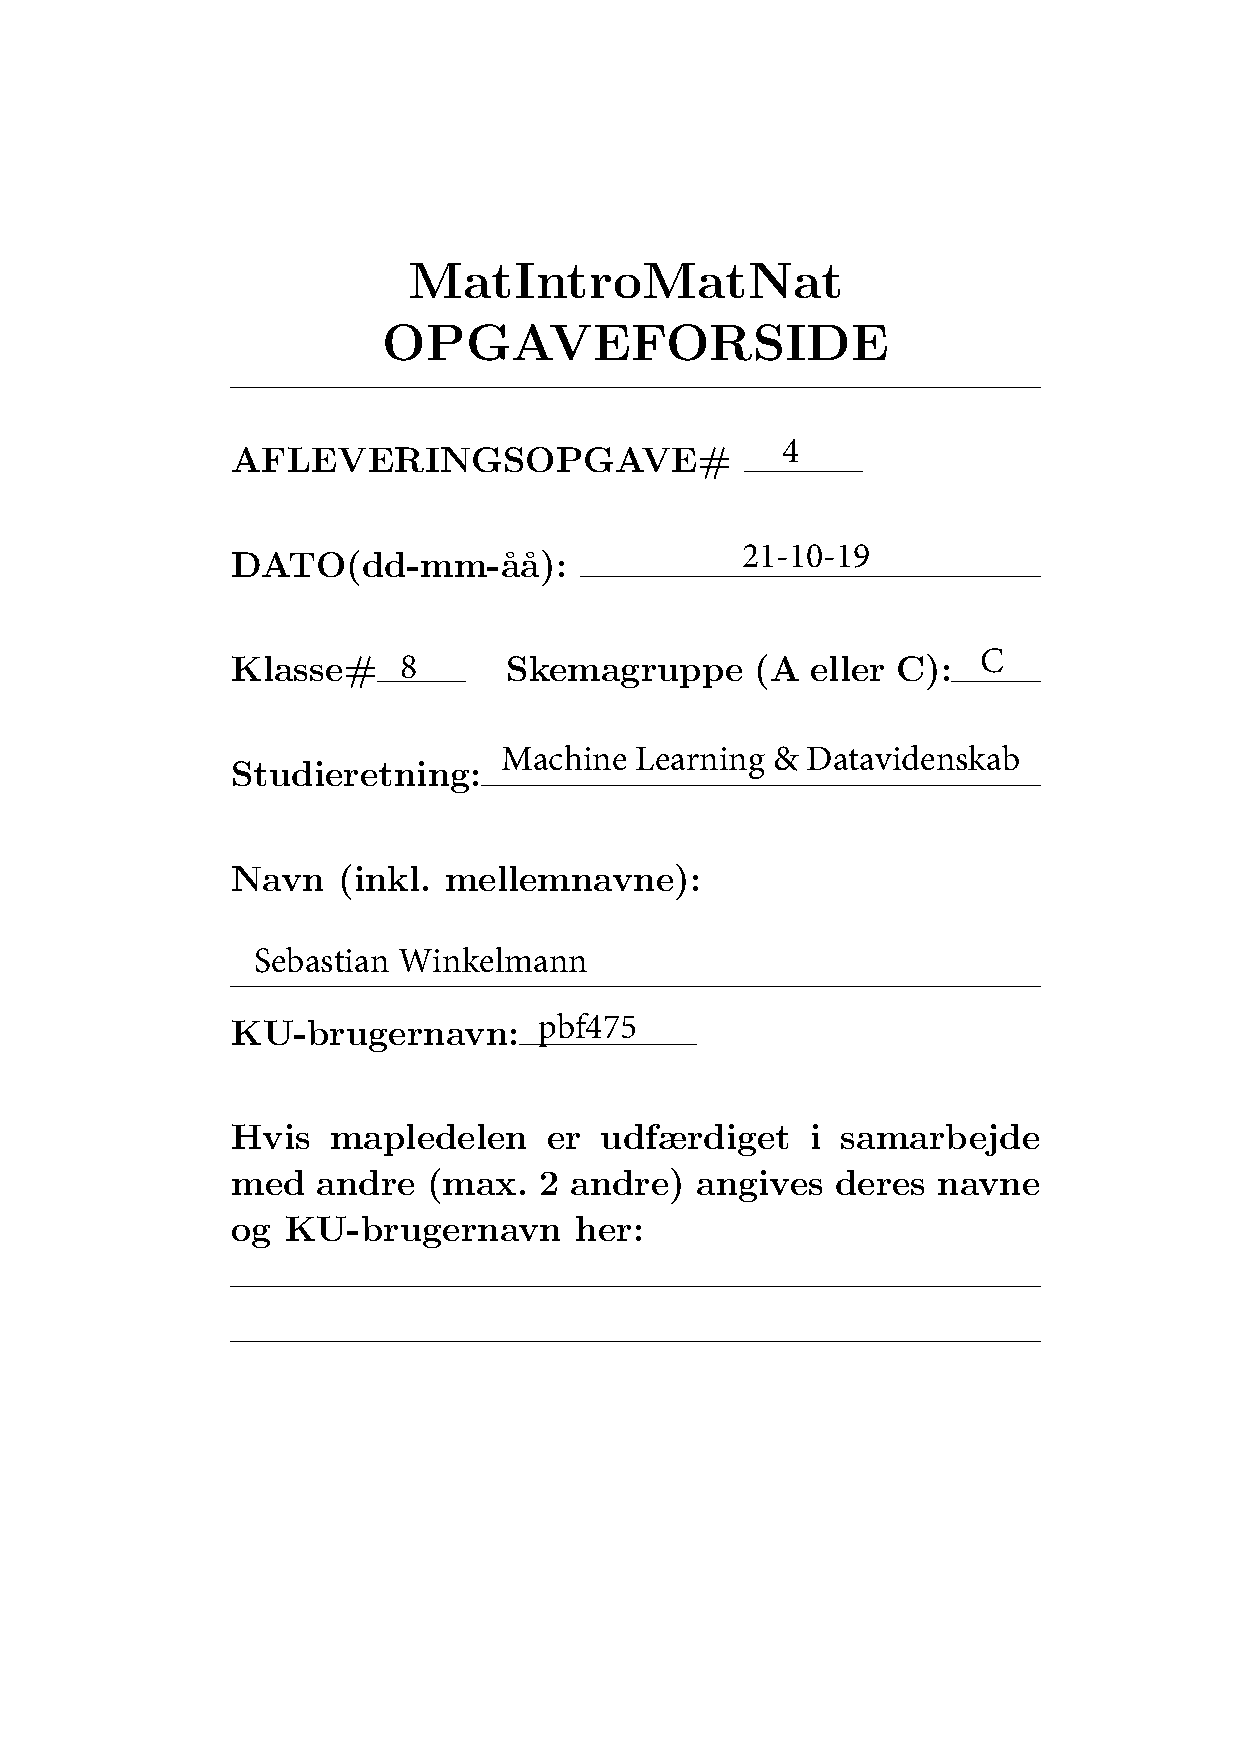
\includepdf{forside.pdf}
\setcounter{chapter}{4}
\section{Partielt afledte}
Jeg tager først den partielle afledede ved $\frac{\partial^2f}{\partial y\partial x}$ og derefter $\frac{\partial^2f}{\partial x\partial y}$
\subsection{$f(x,y)=y^2(1+4xy)$}
\begin{align}
    \frac{\partial^2}{\partial y\partial x} f(x,y)&=\frac{\partial}{\partial y}\left(\frac{\partial}{\partial x}y^2(1+4xy)\right)=\frac{\partial}{\partial y}\left(y^2(4y)\right)\\
    \frac{\partial^2}{\partial y\partial x} f(x,y)&=\frac{\partial}{\partial y}4y^3=12y^2
\end{align}
\begin{align}
    \frac{\partial^2}{\partial x\partial y} f(x,y)&=\frac{\partial}{\partial x}\left(\frac{\partial}{\partial y}y^2(1+4xy)\right)=\frac{\partial}{\partial x}\left(2y(1+4xy)+y^2(4x)\right)\\
    \frac{\partial^2}{\partial x\partial y} f(x,y)&=\frac{\partial}{\partial y}2y+8y^2x+4y^2x=12y^2
\end{align}
\subsection{$g(x,y)=xy+2\cos{(4x+y)}$}
\begin{align}
    \frac{\partial^2}{\partial x\partial y}&=\frac{\partial}{\partial x}\left(\frac{\partial}{\partial y}\left(xy+2\cos{(4x+y)}\right)\right)= \frac{\partial}{\partial x}\left(x-2\sin{(4x+y)}\right)\\
    \frac{\partial^2}{\partial x\partial y}&=\frac{\partial}{\partial x}\left(x-2\sin{(4x+y)}\right)=1-8\cos{(4x+y)}
\end{align}
\begin{align}
    \frac{\partial^2}{\partial y\partial x}&=\frac{\partial}{\partial y}\left(\frac{\partial}{\partial x}\left(xy+2\cos{(4x+y)}\right)\right)= \frac{\partial}{\partial y}\left(y-8\sin{(4x+y)}\right)\\
    \frac{\partial^2}{\partial y\partial x}&=\frac{\partial}{\partial y}\left(y-8\sin{(4x+y)}\right)=1-8\cos{(4x+y)}
\end{align}{}
\subsection{$h(x,y)=2x\ln{(x^2-4y)}$}
\begin{figure}[H]
    \centering
    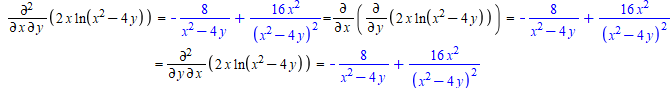
\includegraphics[scale=0.8]{41.png}
    \label{fig:41}
    \caption{Udregning i Maple}
\end{figure}
Når man tager den partielle afledede $\frac{\partial^2}{\partial x_1\partial x_2}f(x_1,x_2)$ differentieres der først med hensyn til $x_2$ (og man behandler $x_1$ som en konstant), for derefter at differentiere den afledede med hensyn til $x_1$ (hvor $x_2$ er en konstant).\par Der tegner sig desuden det mønster at rækkefølgen af partiel differentiation er redundant (kommutativt egenskab). Der gælder altså at $$\frac{\partial^2}{\partial x\partial y} f(x,y)=\frac{\partial^2}{\partial y\partial x} f(x,y)\quad\text{      eller     }\quad\frac{\partial^2f(x,y)}{\partial x\partial y}=\frac{\partial^2f(x,y)}{\partial y\partial x}$$

\section{Kontinuitet}
\begin{equation}
    h(x,y)=\frac{\cos{x}-\cos{y}}{2(x^2+y^2)},\quad h:\mathbb{R}^2\setminus\{(0,0)\}\to\mathbb{R}
\end{equation}
\subsection*{Bestem $H(x):=\lim_{y\to0}h(x,y),\quad x\in\mathbb{R}$}
Lad os bestemme grænseværdien $H$:
\begin{align}
    H(x)&=\lim_{y\to0}h(x,y)=\frac{\cos{x}-\lim_{y\to0}\cos{y}}{2(x^2+\lim_{y\to0}y^2)}=\frac{\cos{x}-1}{2x^2},\text{ for }x\neq0
\end{align}
Vi observerer at 4.10 er en sammensat funktion: $f(x)=\cos{x}-1$ og $g(x)=2x^2$. Da både $f$ og $g$ er kontinuerte funktioner må også $H$ være kontinuert for alle $x\neq0$. Lad os se på den situation hvor $x=0$ (vi tager grænseværdien og benytter L'Hôpitals regel på 0/0-udtryk to gange).
\begin{equation}
    H(0)=\lim_{y\to0}h(0,y)=\lim_{y\to0}\frac{-\cos{y}}{2y^2}=\lim_{y\to0}\frac{-(\cos{y})'}{2(y^2)'}=\lim_{y\to0}\frac{\sin{y}}{4y}=\lim_{y\to0}\frac{\cos{y}}{4}=\frac{1}{4}
\end{equation}
Således er $H$ defineret, selv i $x=0$. Vi skal nu finde ud af hvad grænseværdien af $H(x)$ er:\begin{equation}
    \lim_{x\to0}H(x)=\lim_{x\to0}\frac{(\cos{x}-1)'}{(2x^2)'}=\\lim_{x\to0}frac{(-\sin{x})'}{(4x)'}=\lim_{x\to0}\frac{-\cos{x}}{4}=-\frac{1}{4}
\end{equation}
Sammenholder vi resultaterne for 4.11 og 4.12, da der vi at $\lim_{x\to0}H(x)\neq H(0)$, hvorfor $H(x)$ ikke er kontinuert. Det samme må nødvendigvis gælde for $h(x,y)$, hvorfor en $c=h(0,0)$ ikke findes. Ej heller er $\lim_{(x,y)\to(0,0)}h(x,y)$ defineret da grænseværdien afhænger om man tager den af $x$- eller $y$-aksen ($\lim_{x\to0}\lim_{y\to0}h\neq\lim_{y\to0}\lim_{x\to0}h$).


\section{Toningsopgave -- Taylor og $\arcsin{x}$}
$$(\arcsin)'(x)=\frac{1}{\sqrt{1-x^2}}$$
\subsection{$T_3f$ omkring $a=0$ for $f=\arcsin$}
Taylorpolynomiet for $\arcsin$ vil have følgende forskrift
\begin{align}
    T_3f&=\arcsin{0}+\left(\arcsin\right)'(0)\cdot x+\left(\arcsin\right)''(0)\cdot\frac{x^2}{2}+\left(\arcsin\right)^{(3)}(0)\cdot\frac{x^3}{6}
\end{align}
Vi finder differentialkvotienterne fra 4.13. Bruger potensregel og produktregel.
\begin{align*}
    (\arcsin{x})'&=\frac{1}{\sqrt{1-x^2}}\\
    (\arcsin{x})''&=\left(\frac{1}{\sqrt{1-x^2}}\right)'=\left((1-x^2)^{-\frac{1}{2}}\right)'=x(1-x^2)^{-\frac{3}{2}}=\frac{x}{\sqrt{1-x^2}^3}\\
    (\arcsin{x})'''&=\left(x(1-x^2)^{-\frac{3}{2}}\right)'=(1-x^2)^{-\frac{3}{2}}+x\frac{2x\cdot3}{2}(1-x^2)^{-\frac{5}{2}}=\frac{1}{\sqrt{1-x^2}^3}+\frac{3x^2}{\sqrt{1-x^2}^5}
\end{align*}Da 
$$T_3f=0+\frac{1}{\sqrt{1}}x+\frac{0}{\sqrt{1}^3}\frac{x^2}{2}+\left(\frac{1}{\sqrt{1}^3}+\frac{3(0)^2}{\sqrt{1}^5}\right)\frac{x^3}{6}=x+\frac{x^3}{6}$$
\subsection{Tilnærmelse af $\pi$}
Vi indsætter $x=\frac{1}{2}$ i $T_3f$:\begin{equation}
    b=T_3f\left(\frac{1}{2}\right)=\frac{1}{2}+\frac{1}{8\cdot6}=\frac{24}{48}+\frac{1}{48}=\frac{25}{48}
\end{equation}
Da $\arcsin$ er $\sin$s inverse, da vil dette på enhedscirklen svare til den vinkel hvor højden/$y$-værdien for punktet er $\frac{1}{2}$ (ved $\theta=30^\circ=\frac{\pi}{6}$). Lad os bestemme $6b=\frac{150}{48}=3.125$. Differensen mellem $\pi$ og $6b$ er $\pi-3.125=0.0166$. Min egen approksimation af $\pi\approx3.14159$, hvorved afvigelsen vil være $3.14159-3.125=0.01659$.

\subsection{Maksimal afvigelse}
\begin{equation}
    |R_n\arcsin{x}|\leq\frac{M}{(n+1)!}|x-a|^{n+1},\text{ for }M\geq|(\arcsin{t})^{(4)}|
\end{equation}{}
Da $\arcsin{x}$ og $(\arcsin{x})^{(4)}=\frac{6x^3+9x}{(1-x^2)^{\frac{7}{2}}}$ er kontinuerte for $x\in[0,\frac{1}{2}]$ kan korollaret benyttes. Lad os finde dette $M$. Da vi kigger på intervallet hvor $0\leq t\leq\frac{1}{2}$ vil den 4. afledede ved $t=0$ være 0, mens den antager maksværdien ved $t=\frac{1}{2}$: $\frac{6\cdot\frac{1}{8}+9\cdot\frac{1}{2}}{(\frac{3}{4})^{7/2}}=14.3696$. Benytter man det fundne $M=14.3696$ i 4.15, da får vi at
\begin{equation}
    |R_3\arcsin{x}|\leq\frac{14.3696}{(3+1)!}\left|\frac{1}{2}-1\right|^{3+1}=0.0374208\overline{3}
\end{equation}
Da størrelsen af restledet/afvigelsen for approksimationen $b$ skalerer med $6b$ skal man blot gange resultatet med 6:$$6\cdot0.03742\approx0.2245$$
\begin{figure}[H]
    \centering
    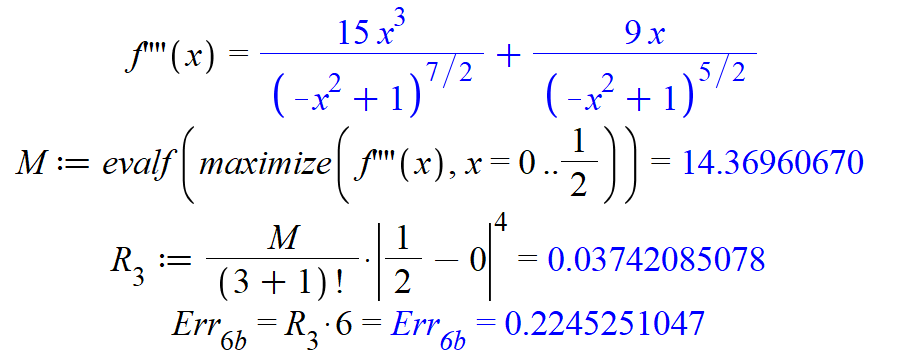
\includegraphics[width=0.6\textwidth]{javaw_IFEFK4Yykw.png}
    \caption{Udregninger i Maple}
\end{figure}
\subsection{Gentagelse af (a)--(c), med $n=100$}
\begin{figure}[H]
    \centering
    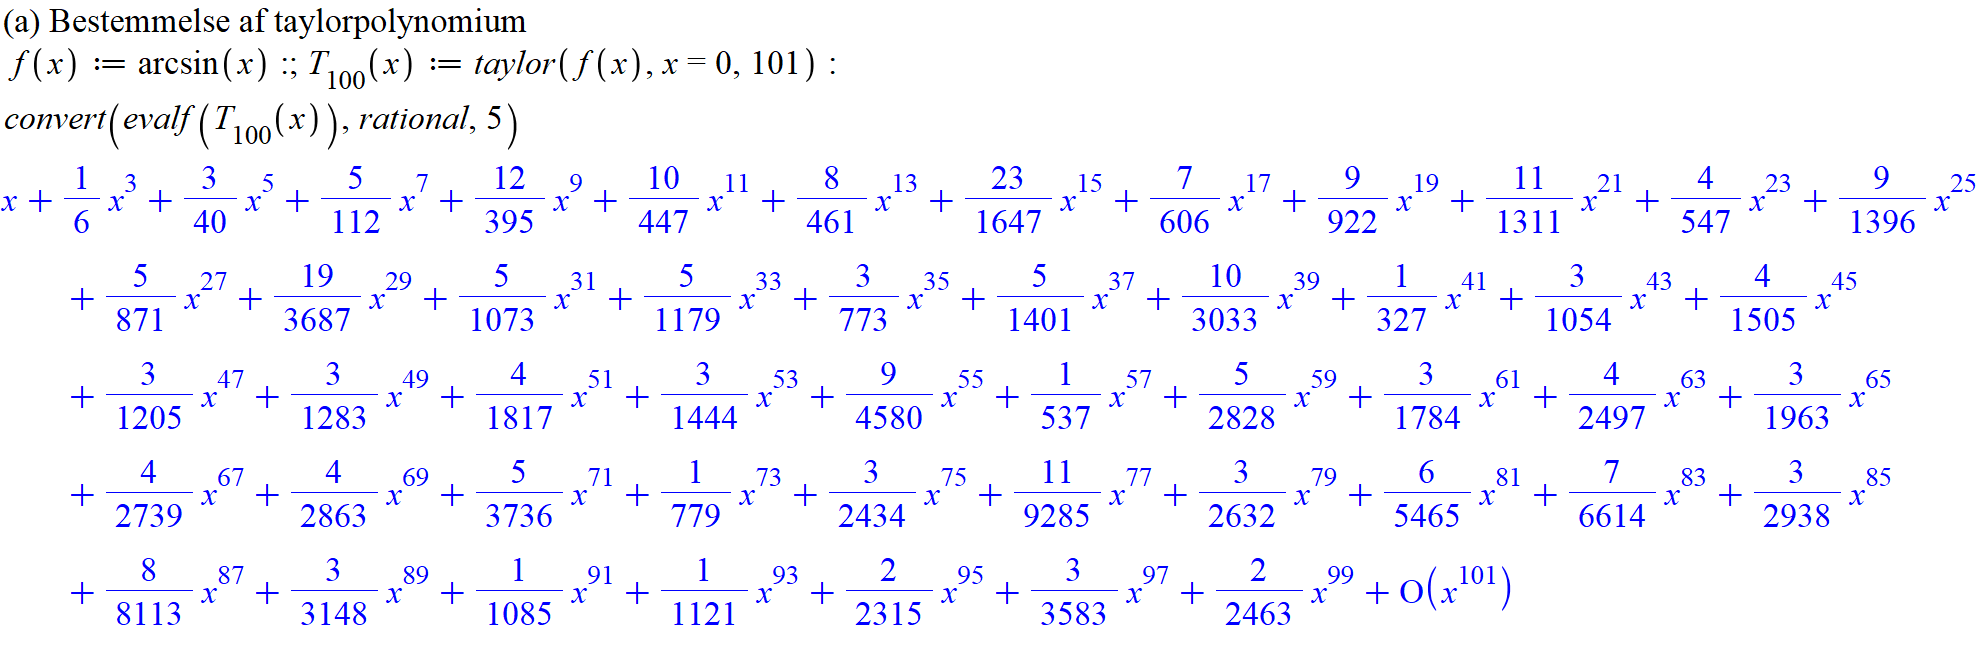
\includegraphics[width=1.2\textwidth]{43da.png}
\end{figure}
Taylorpolynomiet $T_{100}\arcsin{x}$ er altså blevet bestemt. 
\begin{figure}[H]
    \centering
    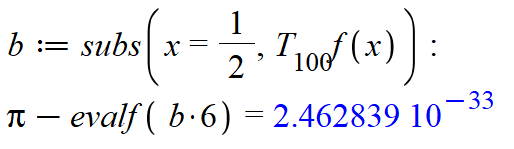
\includegraphics[width=0.36\textwidth]{43db.png}
\end{figure}
Den absolutte afvigelse\footnote{Modsat før finder jeg ikke afvigelsen mellem $T_{100}$ og min egen approksimation $\pi\approx3.14159$ da præcisionen af $T_{100}(\frac{1}{2})$ er så god, at det giver bedre mening at sammenligne den med Maples egen approksimation af $\pi$.} mellem min approksimation og $\pi$ er altså $1.615\cdot10^{-16}$. 
\begin{figure}[H]
    \centering
    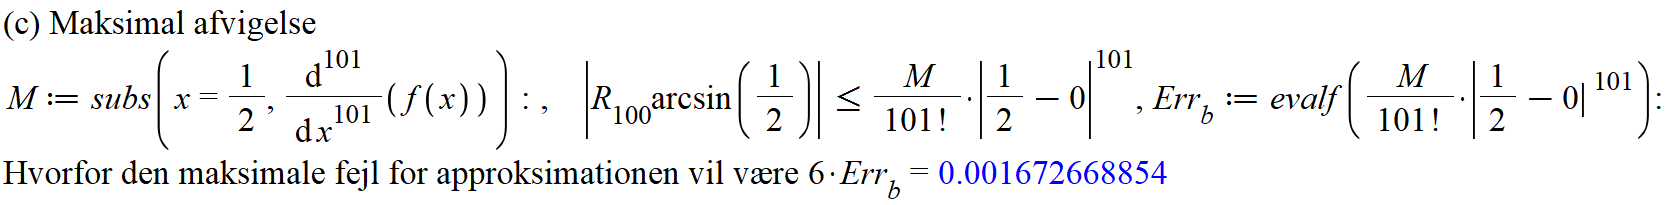
\includegraphics[width=1\textwidth]{43dc.png}
\end{figure}
Den maksimale afvigelse mellem $\pi$ og $6b$ er 0.001673. Det er altså en betydelig ændring i præcision, men på bekostningen af at udtrykkets længden (og kompleksitet) forøges tilsvarende.
\end{document}